\begin{figure}[htbp]
\centering
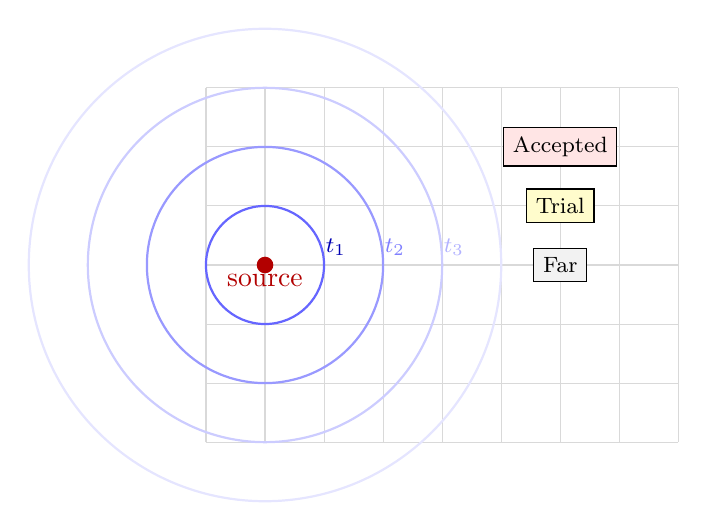
\begin{tikzpicture}[scale=0.75]
  \draw[gray!30,thin] (0,0) grid[step=1] (8,6);
  \fill[red!70!black] (1,3) circle (4pt) node[below] {source};
  \draw[blue!60,thick] (1,3) circle (1);
  \draw[blue!40,thick] (1,3) circle (2);
  \draw[blue!20,thick] (1,3) circle (3);
  \draw[blue!10,thick] (1,3) circle (4);
  \node[blue!70!black,font=\footnotesize] at (2.2,3.3) {$t_1$};
  \node[blue!50,font=\footnotesize] at (3.2,3.3) {$t_2$};
  \node[blue!30,font=\footnotesize] at (4.2,3.3) {$t_3$};
  \node[draw,rectangle,fill=red!10,font=\footnotesize] at (6,5) {Accepted};
  \node[draw,rectangle,fill=yellow!20,font=\footnotesize] at (6,4) {Trial};
  \node[draw,rectangle,fill=gray!10,font=\footnotesize] at (6,3) {Far};
\end{tikzpicture}
\caption{Fast Marching Method: the wavefront propagates from the source. Points are categorized as Accepted, Trial, or Far.}
\label{fig:fast_marching}
\end{figure}
